\chapter{Performance Evaluation of Big Data Processing Strategies for
Neuroimaging}~\label{chp:bigdatastrategies}

% Val\'erie Hayot-Sasson$^{1}$, Shawn T Brown$^{2}$, and Tristan Glatard$^{1}$ \\
% \begingroup \footnotesize $^1$ Department of Computer Science and Software
% Engineering, Concordia University, Montreal, Canada \\
% $^2$ Montreal Neurological Institute, McGill University, Montreal, Canada \\
% \endgroup 
% \vspace{5pt} \\
% Published in: \\
% \hspace*{10pt} \textit{2019 19th IEEE/ACM International Symposium on Cluster,
% Cloud and Grid Computing (CCGRID):} \url{10.1109/CCGRID.2019.00059}


\noindent
Published in: \\
Val\'erie Hayot-Sasson, Shawn T Brown, and Tristan Glatard. Performance Evaluation of Big Data Processing Strategies for
Neuroimaging. \textit{2019 19th IEEE/ACM International Symposium on Cluster,
Cloud and Grid Computing (CCGRID)}. \url{10.1109/CCGRID.2019.00059}



\section{Abstract}
    Neuroimaging datasets are rapidly growing in size as a result of
    advancements in image acquisition methods, open-science and data sharing.
    However, the adoption of Big Data processing strategies by neuroimaging
    processing engines remains limited. Here, we evaluate three Big Data
    processing strategies (in-memory computing, data locality and lazy
    evaluation) on typical neuroimaging use cases, represented by the BigBrain
    dataset. We contrast these various strategies using Apache Spark and Nipype
    as our representative Big Data and neuroimaging processing engines, on Dell
    EMC's Top-500 cluster. Big Data thresholds were modeled by comparing the
    data-write rate of the application to the file system bandwidth and number of
    concurrent processes. This model acknowledges the fact that page caching
    provided by the Linux kernel is critical to the performance of Big Data
    applications. Results show that in-memory computing alone speeds-up
    executions by a factor of up to 1.6, whereas when combined with data
    locality, this factor reaches 5.3. Lazy evaluation strategies were found to
    increase the likelihood of cache hits, further improving processing time.
    Such important speed-up values are likely to be observed on typical image
    processing operations performed on images of size larger than \SI{75}{\giga\byte}. A
    ballpark speculation from our model showed that in-memory computing alone
    will not speed up current functional MRI analyses unless coupled with data
    locality and processing around 280 subjects concurrently. Furthermore, we
    observe that emulating in-memory computing using in-memory file systems
    (\gls{tmpfs}) does not reach the performance of an in-memory engine, presumably
    due to swapping to disk and the lack of data cleanup. We conclude that Big
    Data processing strategies are worth developing for neuroimaging
    applications. 

\section{Introduction} % 1 page with abstract

Big Data processing engines have significantly improved the performance of Big
Data applications by diminishing the amount of data movement that occurs during
the execution of an application. Locality-aware scheduling, introduced by the
MapReduce~\cite{dean2008mapreduce} framework, reduced the overall costs
associated to network transfer of data by scheduling tasks to the nodes located
nearest to the data. Reduction of data movement was further improved upon
through in-memory computing~\cite{zaharia2016apache}, which ensures that data is
maintained in memory between tasks whenever possible. To further reduce the cost
of data movement, lazy evaluation, the process of performing computations only
when invoked, was leveraged by Big Data frameworks to enable further
optimizations such as regrouping of tasks and computing only what is necessary.

Frameworks such as MapReduce and Spark~\cite{zaharia2016apache} have become
mainstream tools for data analytics, although many others, such as
Dask~\cite{rocklin2015dask}, are emerging. Meanwhile, several scientific domains
including bioinformatics, physics or astronomy, have entered the Big Data era
due to increasing data volumes and variety. Nevertheless, the adoption of Big
Data engines for scientific data analysis remains limited, perhaps due to the
widespread availability of scientific processing engines such as
Pegasus~\cite{deelman2005pegasus} or Taverna~\cite{oinn2004taverna}, and the
adaptations required in Big Data processing engines for scientific computing. 

Scientific applications differ from typical Big Data use cases, which might
explain the remaining gap between Big Data and scientific engines. While Big
Data applications mostly target text processing (e.g. Web search, frequent
pattern mining, recommender systems~\cite{leskovec2014mining}) implemented in
consistent software libraries, scientific applications often involve binary data
such as images and signals, processed by a sequence of
command-line/containerized tools using a mix of programming languages (C,
Fortran, Python, shell scripts), referred to as workflows or pipelines. With
respect to infrastructure, Big Data applications commonly run on clouds or
dedicated commodity clusters with locality-aware file systems such as the Hadoop
Distributed File System (HDFS~\cite{shvachko2010hadoop}), whereas scientific
applications are usually deployed on large, shared clusters where data is
transferred between data and compute nodes through shared file systems such as
Lustre~\cite{schwan2003lustre}. Such differences in applications and
infrastructure have important consequences. To mention only one, in-memory
computing requires instrumentation to be applied to command-line tools. 

Technological advances of the past decade, in particular page caching in the
Linux kernel~\cite{love2010linux}, in-memory file systems (tmpfs) and
memory-mapped files might also explain the lack of adoption of Big Data engines
for scientific applications. In such configurations, in-memory computing would
be a feature provided by the operating system rather than by the engine itself.
The frontier between these two components is blurred and needs to be clarified.

% https://ntrs.nasa.gov/archive/nasa/casi.ntrs.nasa.gov/20130001600.pdf

Our primary field of interest, Neuroimaging, is no exception to the generalized
rise of data volumes in science due to the joint increase of image resolution
and subject cohort sizes~\cite{van2014human}. Processing engines have been
developed with neuroinformatics applications in mind, for instance
Nipype~\cite{gorgolewski2011nipype} or the Pipeline System for Octave and Matlab
(PSOM~\cite{bellec2012pipeline}). Big Data engines have also been used for
neuroimaging applications, including the Thunder
project~\cite{freeman2014mapping} and in more specific works such
as~\cite{makkie2019fast}. However, no quantitative performance evaluation has
been conducted on neuroimaging applications to assess the added-value of Big
Data engines compared to traditional processing engines.

This paper addresses the following questions:
\begin{enumerate}
\item What is the effect of in-memory computing, lazy evaluation and data
locality on current neuroimaging applications?
\item Can in-memory computing be effectively enabled by the operating system
rather than the data processing engine?
\end{enumerate}

Answers to these questions have important implications.
In~\cite{mehta2017comparative}, a comparative study of Dask, Spark, TensorFlow,
MyriaDB, and SciDB on neuroinformatics use-cases is presented. It concludes that
these systems need to be extended to better address scientific code integration,
data partitioning, data formats and system tuning. We argue that such efforts
should only be conducted if substantial performance improvements are expected
from in-memory computing, lazy evaluation or data locality. On the other hand,
neuroimaging data processing engines are still being developed, and the question
remains whether these projects should just be migrated to Spark, Dask, or other
Big Data engines.

Our study focuses on performance. We intentionally do not compare Big Data and
scientific data processing engines on the grounds of workflow language
expressivity, fault-tolerance, provenance capture and representation,
portability or reproducibility, which are otherwise critical concerns, addressed
for instance in~\cite{samba}. Besides, our study of performance focuses on the
impact of data writes and transfers. It purposely leaves out task scheduling to
computing resources, to focus on the understanding of data writes and movement.
Task scheduling will be part of our discussion, however.

In terms of infrastructure, we focus on the case of High-Performance Computing
(HPC) clusters that are typically available through University facilities or
national computing infrastructures such as \href{xsede.org}{XSEDE},
\href{http://computecanada.ca}{Compute Canada} or
\href{http://www.prace-ri.eu}{PRACE}, as neuroscientists typically use such
platforms. We assume that HPC systems are multi-tenant, that compute nodes are
accessible through a batch scheduler, and that a file system shared among the
compute nodes is available. We intentionally did not consider distributed,
HDFS-like file systems, as initiatives to deploy them in HPC centers, for
instance Hadoop on-demand~\cite{krishnan2011myhadoop}, have not become
mainstream yet.

Our methods, including performance models, processing engines, applications and
infrastructure used are described in Section~\ref{sec:inmem:methods}.
Section~\ref{sec:inmem:results} presents our results which we discuss in
Section~\ref{sec:inmem:discussion} along with the two research questions mentioned
previously. Section~\ref{sec:inmem:conclusion} concludes on the relevance of Big Data
processing strategies for neuroimaging applications.

\section{Materials and Methods} % 4 pages
\label{sec:inmem:methods}

The application pipelines, benchmarks, performance data, and analysis scripts
used to implement the methods described hereafter are all available at
\url{https://github.com/big-data-lab-team/paper-in-mem-locality} for further
inspection and reproducibility. Links to the processing engines and processed
data are provided in the text.

\subsection{Engines} % 1.5 pages

\subsubsection{Apache Spark}

Apache Spark is a well-established Scala-based processing framework for Big
Data, with APIs in Java, Python and R. Its generalized nature allows Spark to
not only be applied to batch workflows, but also SQL queries, iterative machine
learning applications, data streaming and graph processing. Spark's main
features include data locality, in-memory processing and lazy evaluation, which
it achieves through its principle abstraction, the Resilient Distributed Dataset
(RDD). 

An RDD is an immutable parallel data structure that achieves fault-tolerance
through the concept of lineage~\cite{zaharia2010spark}. Rather than permitting
fine-grained transformations, only coarse-grained transformations (applying to
many elements in the RDD), can be applied, thereby making it simple to maintain
a log of data modifications. This log, known as the lineage, is used to
reproduce any lost data modifications.

Two types of operations can be performed on RDDs: transformations and actions.
Applying a transformation to an RDD produces a new child RDD through a narrow or
wide dependency. A narrow dependency signifies that the child is only dependent
on a single parent partition, whereas a child RDD is dependent on all parent
partitions in a wide dependency. Examples of transformations include map, filter
and join. To materialize an RDD, an action must be performed, such as a reduce
or a collect. Lazy evaluation is represented in Spark through the use of
transformations and actions. A series of transformations may be defined without
the data ever being materialized. Using this strategy, Spark can optimize data
processing throughout the application.

All actions and wide dependencies require a shuffle -- Spark's most costly
operation. Every shuffle begins with each map task saving its data to local
files for fault tolerance. The shuffle operation then redistributes the data
across the partitions as requested. A shuffle marks a stage boundary in Spark,
where reduce-like operations will not begin until all dependent map tasks have
completed.

Although Spark uses in-memory computing, it is not necessary for all the data to
fit in memory. Spark will spill any RDD elements that cannot be maintained in
memory to disk. Moreover, as Spark transformations generate new RDDs and
numerous transformations may occur within a single application, Spark implements
a Least-Recently Used (LRU) eviction policy. If an evicted RDD needs to be
reused, Spark will recompute it using the lineage data collected. As
demonstrated in~\cite{freeman2014mapping}, caching significantly improves
processing times of iterative algorithms where RDDs are reused. It can be of
even greater importance if the RDD is costly to recompute.

Data locality in Spark is achieved through the scheduling of tasks to partitions
which have the data loaded in memory. If the data is instead stored on HDFS, the
scheduler will assign it to one of the preferred locations specified by HDFS.
Spark's scheduler utilizes delay scheduling to optimize fairness and locality
for all tasks.

Three different types of schedulers are compatible with Spark: 1) Spark
Standalone, 2) YARN~\cite{vavilapalli2013apache} and 3)
Mesos~\cite{hindman2011mesos}. The Spark Standalone scheduler is the default
scheduler. The YARN scheduler designed for Hadoop~\cite{white2012hadoop}
clusters and is prepackaged with Hadoop installations, whereas in contrast,
Mesos was designed to be used in multi-tenant cluster environments. In our
experiments, we focus on the Spark Standalone cluster.

Executing Spark applications on HPC systems with Spark-unaware schedulers may be
inefficient. The amount of resources requested by Spark may impede Spark-cluster
scheduling time. Using pilot-scheduling strategies to add nodes to the Spark
cluster as they are allocated by the underlying schedulers may speedup
allocation and overall processing time~\cite{paraskevakos2018pilot}. This,
however, is not studied in the current paper.

As Spark is frequently used by the scientific community, we designed our
experiments using the PySpark API. This is at a cost to performance as the
PySpark code must undergo Python to Java serialization. We used Spark version
2.3.2 installed from \url{https://spark.apache.org}.

\subsubsection{Nipype}

Nipype is a popular Python neuroimaging processing engine. It aims at being a
solution for easily creating reproducible neuroimaging workflows. Although
Nipype does not employ any Big Data processing strategies, it provides plugins
to numerous schedulers found in most clusters readily available to researchers,
such as the Sun/Oracle Grid Engine (SGE/OGE),
\href{http://www.adaptivecomputing.com/products/torque/}{TORQUE},
\href{https://slurm.schedmd.com/}{Slurm} and
\href{https://research.cs.wisc.edu/htcondor/}{HTCondor}. It also includes its
own scheduler, MultiProc, for parallel processing on single nodes. Furthermore,
Nipype provides many built-in interfaces to commonly used neuroimaging tools
that can be incorporated within the workflows. Nipype's ability to easily
parallelize workflows in researcher-available cluster setups, capture detailed
provenance information necessary for reproducibility, and allow users to easily
integrate existing neuroimaging tools, make it preferable over existing Big Data
solutions, which would necessitate modifications to achieve this.

Jobs, or Interfaces in Nipype, are encapsulated by a Node. A Node dictates that
the job will execute on a single input. However, the MapNode, a child variant of
the Node, can execute on multiple inputs. All tasks in Nipype execute in their
own uniquely named subdirectory which facilitates provenance tracking of inputs
and outputs and also enables checkpointing of the workflow. In the case of Node
failure or application modification, only the nodes which have been modified
(verified by hash) or have not successfully completed, are re-executed.

In order for Nipype to operate as intended, a file system shared by all the nodes
is required. However, it is still possible to save to a non-shared local
file system, but it may come at the expense of fault-tolerance, as data located
on failed nodes will be permanently lost. Moreover, the user will need to ensure
that the files are appropriately directed to the nodes that require them as
there is no guarantee of data locality in Nipype.

We used Nipype version 1.1.4 installed through the pip package manager.

\subsection{Data Storage Locations}

Data storage location is critical to the performance of Big Data applications on
HPC clusters. Data may reside in the engine memory, on a file system whose
contents reside in virtual memory (for instance tmpfs), on disks local to the
processing node, or on a shared file system. Table~\ref{table:inmem:features}
summarizes the Big Data strategies that can be used depending on the data
location. In addition, lazy evaluation is available in Spark regardless of data
location. The remainder of this Section explains this Table and provides related
performance models.

\begin{table}
\centering
\begin{tabular}{c|cc}
   \rowcolor{headcolor}
    Data Location                 & In-Memory     & Data Locality        \\
    \rowcolor{headcolor}
                                  & Computing     &                     \\
                                  \hline          
In-memory                         & \cellcolor{green!25} Yes           &
\cellcolor{green!25}Yes                      \\
tmpfs                             & \cellcolor{green!25} Yes           &
\cellcolor{green!25}Yes                  \\
Local Disk                        & \cellcolor{orange!25}Page Caching  &
\cellcolor{green!25}Yes                  \\
Shared File System                & \cellcolor{orange!25}Page Caching  &
\cellcolor{red!25}No                
\end{tabular}
\setlength{\belowcaptionskip}{-10pt}
\caption{Big Data strategies on a shared HPC cluster.}
\label{table:inmem:features}
\end{table}

\subsubsection{In-Engine-Memory and In-Memory File System} 

 The main difference between storing the data in the engine memory, as in Spark,
 and simply writing to an in-memory file system, such as tmpfs, is what happens
 when the processed data fills up the available memory. When engine memory is
 used, the engine must clean up unused data to avoid crashes. When an in-memory
 file system is used, the user is responsible ensuring that the file system does
 not reach capacity. Should it be necessary to free up additional memory, the
 kernel will swap file system memory to disk and the performance will become that
 of local disk writes. In our experiments, we will explore the configuration
 where the data consumed by the application approaches the threshold of
 available memory.

\subsubsection{Local Disk} % 0.5 page

% Perhaps refer to this: https://ieeexplore.ieee.org/abstract/document/5496998

Storing data on local disks inevitably enables data locality, since data
transfers are not necessary when tasks are executed on the nodes where the data
resides. However, in absence of a more specific file system such as HDFS to
handle file replication across computing nodes, data locality comes at the price
of stringent scheduling restrictions, as tasks can only be scheduled to the
single node that contains their input data.


The performance of local disk accesses is strongly dependent on the page caching
mechanism provided by the Linux kernel, described in    
details in~\cite{love2010linux}. To summarize, data read from disk remains
cached in memory until evicted by an LRU (Least Recently Used) strategy. When a
process invokes the \texttt{read()} system call, the kernel will return the data
directly from memory if the requested data lies in the \gls{pc}, realizing a
cache \emph{hit}. Cache hits drastically speed-up data reads, by masking the
disk latency and bandwidth behind a memory buffer. In effect, page caching
provides in-memory computing transparently to the processing engine. However,
page cache eviction strategies currently cannot be controlled by the
application, which prevents processing engines from anticipating reads by
preloading the cache. Scheduling strategies might be designed to maximize cache
hits, however. For instance, lazy evaluation could result in more cache hits by
scheduling data-dependent tasks on the same node.

Page caching has a more dramatic effect on disk writes, reducing their duration
by several orders of magnitude. When a process calls the \texttt{write()} system
call, data is copied to a memory cache that is asynchronously written to disk by
flusher threads, when memory shrinks, when ``dirty" (unwritten) data grows, or
when a process invokes the \texttt{sync()} system call. This asynchronous
flushing of the page cache is called \emph{writeback}.
%~ It should be noted that writeback may lead to data ~ loss in case of system
%failure. 

Page caching is essentially a way to emulate in-memory computing at the kernel
level, without requiring a dedicated engine. The size of the page cache,
however, becomes a limitation when processes write faster than the disk
bandwidth. When this happens, the page cache rapidly fills up and writes are
limited by the disk write bandwidth as if no page cache was involved.

We introduce the following basic model to describe the filling and flushing of
the page cache by an application:
$$
d(t) = \left( \frac{D}{C} - \frac{\delta}{\gamma} \right)t + d_0,
$$
where:
\begin{itemize}
\item $d(t)$ is the amount of data in the page cache at time t
\item $D$ is the total amount of data written by the application
\item $C$ is the total CPU time of the application
\item $\delta$ is the disk bandwidth
\item $\gamma$ is the max number of concurrent processes on a node
\item $d_0$ is the amount of data in the page cache at time $t_0$
\end{itemize}

This model applies to parallel applications assuming that (1) concurrent
processes all write the same amount of data, (2) concurrent processes all
consume the same CPU time, (3) data is written uniformly along task execution.
With these assumptions, all the processes will write at the same rate, which
explains why the model does not depend on the total number of concurrent
processes in the application, but only on the max number of concurrent processes
executing on the same node ($\gamma$). While these assumptions would usually be
violated in practice, this simple model already provides interesting insights on
the performance of disk writes, as shown later. Naturally, the model also
ignores other processes that might be writing to disk concurrently to the
application, which we assume negligible here. 

In general, an application should ensure that $\dot d$ remains negative or null,
leading to the following inequality:
\begin{equation}
\frac{D}{C} \leq \frac{\delta}{\gamma} \label{eq:inmem:page-cache-inequality}
\end{equation}
This defines a D/C (data-write) rate beyond which the page cache becomes
asymptotically useless. It should be noted that the transient phase during which
the page cache fills up might last a significant amount of time, in particular
when $\dot d$ is positive and small. We intentionally do not model the transient
phase as it requires detailed knowledge of difficult to estimate parameters  
such as the page cache size and the initial amount of data in it ($d_0$).

 We will use Equation~\ref{eq:inmem:page-cache-inequality} to define our benchmarks
and interpret the results. It should be noted that leveraging the page cache,
and therefore ensuring that Equation~\ref{eq:inmem:page-cache-inequality} holds, has
important performance implications: with page caching, the write throughput will
be that of memory, while without page caching it will be that of the disk.

% Cache eviction: LRU/n.

\subsubsection{Shared File System}

We model a shared file system using its global realized bandwidth $\Delta$,
shared by all concurrent processes in the cluster. We are aware that such a
simplistic model does not describe at all the intricacies of systems such as
Lustre. In particular, metadata management, RPC protocol optimizations and
storage optimizations are all covered under the realized bandwidth. We do,
however, consider the effect of page caching in shared file systems, since in
Linux writes to network-mounted volumes benefit from this feature too.

As in the local disk model, we note that page caching will only be useful when
the flush bandwidth is greater than the write throughput of the application,
that is:
\begin{equation}
\frac{D}{C} \leq \frac{\Delta}{\Gamma}, \label{eq:inmem:page-cache-sharedfs}
\end{equation}
where $\Gamma$ is the max number of concurrent processes \emph{in the cluster}.
Note that $\frac{\Delta}{\Gamma}$ will usually be much lower than
$\frac{\delta}{\gamma}$.     


% KEEP THIS FOR WHEN WE LOOK AT SIMULATION

%\subsection{Simulation} % is it included? 0.5 page

% \todo{Remove if not included}

% Even if we end up not using simulation, here we should explain why the model
% in simgrid is limited. Refer to Fred's paper at CCGrid 2017. The following
% sub-sections become a set of models that we could implement in simulation to
% make it more realistic.

% Talk about ~\cite{lebre2015adding} and \cite{wrench}. Most simulation toolkits
%  have focused on task scheduling. And
%  https://dl.acm.org/citation.cfm?id=3041715

\subsection{Infrastructure} % 1/4 a page (half a col)

 All experiments were executed on
 \href{https://www.dellemc.com/resources/en-us/asset/sales-documents/products/storage/h16221-hpc-lab-brochure.pdf}{Dell
 EMC's Zenith cluster}, a Top-500 machine in the
 \href{https://www.dellemc.com/en-us/solutions/high-performance-computing/HPC-AI-Innovation-Lab.htm}{Dell
 EMC HPC and AI Innovation Lab}, running Slurm. For the Spark experiments, a
 Spark cluster was started on a Slurm allocation comprised of 16 dedicated
 nodes. Each Compute node has Red Hat Enterprise Linux Server release 7.4
 (Maipo) as the base operating system with kernel version
 3.10.0-693.17.1.el7.x86\_64 (patched for Spectre/Meltdown). Dell EMC PowerEdge
 C6420 with dual Intel Xeon Gold 6148/F processors (40 cores per node) and 192GB
 ($12\times16$~GB), 2666 MHz memory, serve as the compute nodes. Each compute
 has a 120GB M.2 SATA SSD as local disk. A Dell HPC Lustre Solution with a raw
 storage of 960TB is accessible on each compute node through a 100~Gb/s Intel
 OmniPath network. All the nodes connect to a director switch in a 1:1
 non-blocking topology. The realized write bandwidth of the local disk, Lustre
 file system and tmpfs were measured by sequentially writing various numbers of
 image blocks containing random intensities, to avoid caching effects (see:
 \href{https://github.com/big-data-lab-team/paper-in-mem-locality/blob/master/benchmark_scripts/measure_bandwidth.py}{measure\_bandwidth.py}).
 They are reported in Table~\ref{table:inmem:bdwdths}.

\begin{table}
\centering
\begin{tabular}{c|c}
\rowcolor{headcolor}
Data location & Measured write bandwidths (MB/s)\\
\hline
tmpfs                 & 1377.18 \\
Local disk ($\delta$) & 193.64  \\
Lustre   ($\Delta$)   & 504.03 \\
\end{tabular}
\setlength{\belowcaptionskip}{-10pt}
\caption{Measured bandwidths}
\label{table:inmem:bdwdths}
\end{table}

\subsection{Datasets} % 1/4 of a page (half a col)

We used BigBrain~\cite{amunts2013bigbrain}, a 75GB 40$\mu$m isotropic
histological image of a 65-year-old human brain. The BigBrain was selected due
to its uniqueness, as there does not yet exist a higher-resolution image of a
human brain. Moreover, there currently exists a lack of standardized tools for
processing the BigBrain as a consequence of its size. To examine the effects
processing the BigBrain has on Big Data strategies, we partitioned the full
$3845\times3015\times3470$ voxel image into 30 ($5\times3\times2$) chunks, 125
($5\times5\times5$) chunks and 750 ($5\times15\times10$) chunks. Additionally,
the full image was also split in half ($769\times603\times347$ voxels) and the
half image was partitioned into 125 chunks.

Processing large images is only considered to be part of the Big Data problem in
neuroscience. The other problem being the processing large MRI datasets, that
is, datasets consisting of many small brain images belonging to various
different subjects. This situation is commonly observed in functional MRI
(fMRI), where it is becoming increasingly common to process data from hundreds
of subjects. Although we have not explored explicitly the processing of large
MRI datasets, the 75GB BigBrain is within the size ballpark~\cite{van2014human}
of MRI datasets commonly processed in today's studies.

Since both small and large datasets may need to be processed using the same
analysis pipeline, we examined the effects of the data management strategies on
small data as well. For this, we selected a 12MB T1W image belonging to subject
1 of OpenNeuro's
\href{https://openneuro.org/datasets/ds000001/versions/00006/file-display/sub-01:anat:sub-01_T1w.nii.gz}{ds000001
dataset version 6}. In order to split the image into 125 equal-sized chunks, it
was necessary to zero-pad the image to the dimensions $165\times200\times200$
voxels, which subsequently increased the total image size to 13MB.

\subsection{Applications} % 1 page
\begin{algorithm2e}\caption{Incrementation}\label{alg:inmem:incrementation}
\SetAlgoLined \SetKwInOut{Input}{Input} \Input{$x$ a sleep delay in seconds;\\
           $n$ a number of iterations;\\
           $C$ a list of paths to cache locations;\\
           $fs$ filesystem to write to (mem, tmpfs, local disk, Lustre);\\}
    \ForEach{$chunk \in C$}{ read $chunk$ from Lustre \For{$i \in [1, n]$}{
    $chunk \gets chunk+1$\; sleep $x$\; \If{$i < n$} {save $chunk$ to $fs$\;} }
    save $chunk$ to Lustre }
\end{algorithm2e}

To effectively investigate how the different strategies impact processing, we
selected a simple incrementation pipeline (Algorithm~\ref{alg:inmem:incrementation})
that consists exclusively of map stages. A series of map-only stages would
enable us to evaluate the effects of in-memory computing when data locality is
preserved. Incrementation was selected over other applications, such as
binarization, as it ensured that a new image was created at each step (i.e. no
caching effects within the executing application). Each partitioned chunk was
incremented by 1, in parallel, by each task. As incrementing images is not a
time-consuming process, we added a sleep delay to the tasks to study the effects
of tasks duration. The incremented chunks would be either maintained in-memory
(Spark only) or saved to either tmpfs, local disk or Lustre (Spark and Nipype).
Should more than a single iteration be requested, the incremented chunks would
be incremented again and saved to the same file system. This would repeat until
the number of requested iterations had elapsed. In all conditions, the first
input chunks and final output chunks would reside on Lustre. We chose to perform
our initial input/final output on Lustre as local storage is typically only
accessible to a user for the duration of the execution in HPC environments.

\subsection{Experiments}

We conducted four experiments in which we varied (1) the number of iterations in
the application ($n$ in Algorithm~\ref{alg:inmem:incrementation}), (2) the
task duration ($x$), (3) the chunk size given a constant image size, (4) the
total image size. To evaluate the page-cache model, experiment conditions fell
in different regions of Equations~\ref{eq:inmem:page-cache-inequality}
and~\ref{eq:inmem:page-cache-sharedfs}, as summarized in
Table~\ref{table:inmem:experiments}. Among the 16 nodes available, 1 was dedicated to
the Spark master and driver, and the remaining 15 were used as compute nodes.
Since data locality is not normally preserved in Nipype (a new Slurm allocation
is requested for each processed task), we instrumented Nipype to ensure data
locality (see:
\href{https://github.com/big-data-lab-team/paper-in-mem-locality/blob/master/benchmark\_scripts/run\_benchmarks.py}{run\_benchmarks.py}).
That is, the chunks were split into partitions, and for each partition, we
requested a Slurm allocation to process the entire pipeline in parallel using
Nipype's MultiProc scheduler on a given node. This was possible as no
communication was required between the processed chunks.

\begin{table*}
\centering
\resizebox{\columnwidth}{!}{%
\begin{tabular}{c|ccc|cccc|cc}
  \rowcolor{headcolor}
  \multicolumn{10}{c}{Experiment 1: Number of Iterations}\\
  \hline
  \rowcolor{headcolor}
 n & D (GB) & C (s) & D/C (MB/s) & $\gamma$ & $\delta/\gamma$ (MB/s) & $\Gamma$
 & $\Delta/\Gamma$ (MB/s)& (D/C)/($\delta/\gamma$) & (D/C)/($\Delta/\Gamma$)\\
 \hline
1   &75    & 430    & 178.6 & 9 & 21.5 & 125 & 4.0 & \cellcolor{red!20} 8.3 &
\cellcolor{red!20} 44.7\\
10  & 750   & 4,300 & 178.6 & 9 & 21.5 & 125 & 4.0 & \cellcolor{red!20} 8.3 &
\cellcolor{red!20} 44.7\\
100 & 7,500 & 43,000& 178.6 & 9 & 21.5 & 125 & 4.0 & \cellcolor{red!20} 8.3 &
\cellcolor{red!20} 44.7\\
\hline
  \multicolumn{10}{c}{}\\

\rowcolor{headcolor}
  \multicolumn{10}{c}{Experiment 2: Task Duration}\\
  \hline
  \rowcolor{headcolor}
 x (s) & D (GB) & C (s) & D/C (MB/s) & $\gamma$ & $\delta/\gamma$ (MB/s) &
 $\Gamma$ & $\Delta/\Gamma$ (MB/s)& (D/C)/($\delta/\gamma$) &
 (D/C)/($\Delta/\Gamma$)\\
 \hline
 2.4  & 750 & 3,000   & 256   & 9 & 21.5 & 125 & 4.0 &  \cellcolor{red!20} 11.9
 & \cellcolor{red!20} 64   \\
 3.44 & 750 & 4,300   & 178.6 & 9 & 21.5 & 125 & 4.0 &  \cellcolor{red!20} 8.3 &
 \cellcolor{red!20} 44.7   \\
 7.68 & 750 & 9,600   & 80    & 9 & 21.5 & 125 & 4.0 &  \cellcolor{red!20} 3.7 &
 \cellcolor{red!20} 20   \\
 320  & 750 & 400,000 & 1.9   & 9 & 21.5 & 125 & 4.0 &  \cellcolor{green!20}
 0.09 & \cellcolor{green!20} 0.48  \\
 \hline
  \multicolumn{10}{c}{}\\
  
 \rowcolor{headcolor}
  \multicolumn{10}{c}{Experiment 3: Number of Chunks}\\
  \hline
  \rowcolor{headcolor}
 chunks & D (GB) & C (s) & D/C (MB/s) & $\gamma$ & $\delta/\gamma$ (MB/s) &
 $\Gamma$ & $\Delta/\Gamma$ (MB/s)& (D/C)/($\delta/\gamma$) &
 (D/C)/($\Delta/\Gamma$)\\
 \hline
 30  & 750 & 4,400   & 174.6 & 2  & 96.8 & 30  & 16.8 &  \cellcolor{red!20} 1.8
 & \cellcolor{red!20} 10.4   \\
 125 & 750 & 4,400   & 174.6 & 9  & 21.5 & 125 & 4.0 &  \cellcolor{red!20} 8.1 &
 \cellcolor{red!20} 43.7  \\
 750 & 750 & 4,400   & 174.6 & 25 & 7.7  & 375 & 1.3 &  \cellcolor{red!20} 22.7
 & \cellcolor{red!20} 134.3  \\

\hline
  \multicolumn{10}{c}{}\\ 
 \rowcolor{headcolor}
  \multicolumn{10}{c}{Experiment 4: Image Size}\\
  \hline
  \rowcolor{headcolor}
 image  & D (GB) & C (s) & D/C (MB/s) & $\gamma$ & $\delta/\gamma$ (MB/s) &
 $\Gamma$ & $\Delta/\Gamma$ (MB/s)& (D/C)/($\delta/\gamma$) &
 (D/C)/($\Delta/\Gamma$)\\
 \hline
 BigBrain      & 750   & 2,200   & 349.1     & 9  & 21.5  & 125 & 4.0 &
 \cellcolor{red!20} 16.2 & \cellcolor{red!20} 87.3   \\
 Half BigBrain & 375   & 2,200   & 174.6     & 9  & 21.5  & 125 & 4.0 &
 \cellcolor{red!20} 8.1 & \cellcolor{red!20} 43.7   \\
 MRI           & 0.127 & 2,200   & 0.06      & 9  & 21.5  & 125 & 4.0 &
 \cellcolor{green!20} 0.003 & \cellcolor{green!20} 0.015  
\end{tabular}
} \caption{Experiment conditions. Red cells denote the conditions where the
inequalities in Equations~\ref{eq:inmem:page-cache-inequality}
and~\ref{eq:inmem:page-cache-sharedfs} do not hold, i.e., the page cache is
asymptotically useless. Green cells show the conditions where the page cache
covers all data writes.}
\label{table:inmem:experiments}
\end{table*}

For our first incrementation experiment, we investigated the effects of Big Data
strategies on varying total data size. To achieve this, we increased the number
of incrementation iterations from 1, 10 and 100 times. The total data size would
then increase from \SI{75}{\giga\byte}, at 1 iteration, to \SI{7,500}{\giga\byte}, at 100 iterations. The
total number of chunks was 125. Chunks all ran concurrently ($\Gamma$=125) and
were equally balanced among 15 nodes, leading to 8 or 9 concurrent jobs per node
($\gamma$=9). Task duration was fixed at 3.44 seconds.

In the second experiment, we evaluated the effects of Big Data strategies on
varying task duration. If the page cache has sufficient time to flush, it would
be expected that in-memory computing and local disk perform equivalently. We
varied the task duration between 2.4 and 320 seconds such that the D/C falls
into different regions of Equations~\ref{eq:inmem:page-cache-inequality}
and~\ref{eq:inmem:page-cache-sharedfs}. The number of chunks was maintained at 125,
leading to $\Gamma$=125 and $\gamma$=9. The number of iterations was fixed to
10.

As a third incrementation experiment, we were interested in the effects of chunk
size on Big Data strategies. Naturally, a greater chunk size signifies a
decrease in parallelism. However, it also signifies an increase in sequential
I/O (increased $\Delta/\Gamma$ and $\delta/\gamma$). For this experiment we
partitioned the complete BigBrain image into 30, 125 and 750 chunks,
corresponding to $\gamma$ values of 2, 9 and 25 respectively. While Spark
attempted to load-balance the data, it used up only 25 of the 40 cores for 750
chunks. In contrast, Nipype tried to use up as many cores as possible. Unlike
the previous experiment, the D/C rate was kept static at 178.6MB/s, however,
this ratio ensured that different regions of the inequality were reached
depending on amount of parallelism. The number of iterations was fixed to 10,
and the task duration was adjusted so that C remained constant at 4,400s.

For our fourth and final incrementation experiment, we investigated the effects
of the strategies on different image sizes. We selected the \SI{75}{\giga\byte} BigBrain, the
\SI{38}{\giga\byte} half BigBrain and the 13M T1W MRI image for this experiment. The number of
chunks was fixed to 125. Similarly to the previous experiment, the total
sequential compute time was fixed (10 iterations, 1.76 seconds per task),
however, due to varying size in total data processed (D), the D/C rate varied.
Once again, we ensured that the D/C rate fell in multiple different regions of
the inequality. The D/C rate ranged from 349.1 MB/s for BigBrain and 174.6MB/s
for half BigBrain, to 0.06MB/s for the MRI image. Only the 0.06MB/s MRI
satisfied the inequality for both Lustre and local disk.


% average (1 shuffle) Nipype: can't use SLURM plugin so had to actively poll.

% kmeans (many shuffles)

% Example BIDS app

% fmriprep?

% Explain how we tweaked scheduling in Nipype to make it similar to Spark,
% otherwise we're only measuring scheduling differences. Needs a discussion on
% scheduling somewhere.

% Talk about our I/O pattern: random I/O, sequential.


\section{Results} % 2 pages
\label{sec:inmem:results}

% We checked that scheduling was similar in both cases (show a two Gantt charts
% to illustrate)

\begin{figure*}

\begin{subfigure}{0.5\columnwidth}
    \centering
    \captionsetup{width=.85\linewidth}
    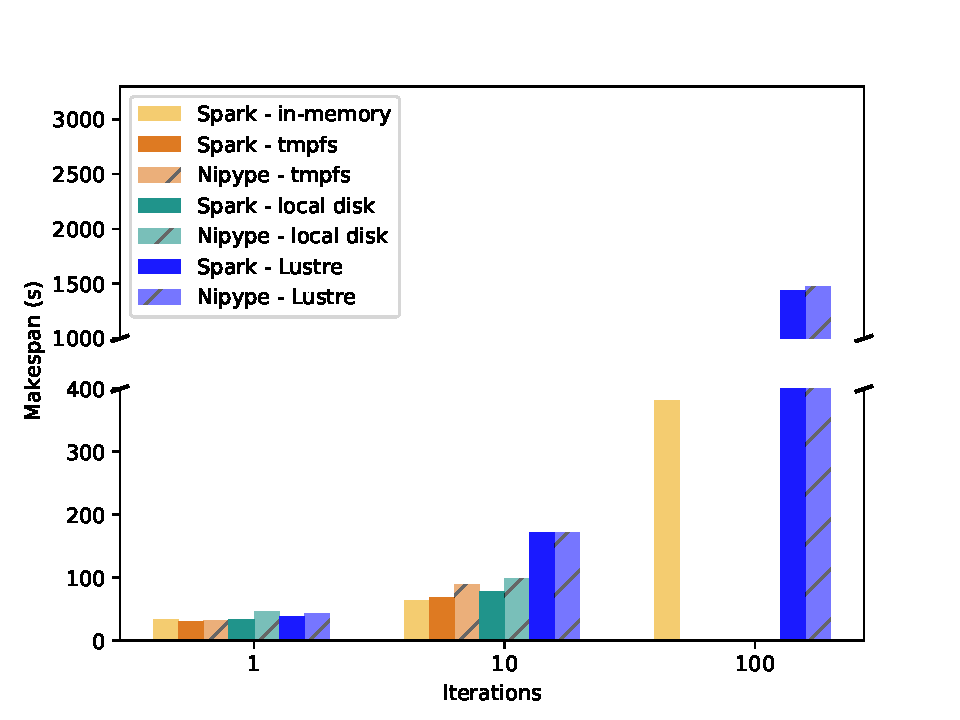
\includegraphics[width=\columnwidth]{figures/inmem/iterations.pdf}%
    \caption{Experiment 1: complete BigBrain, 125 chunks, 3.44-second
    tasks.}\label{fig:inmem:iterations}
\end{subfigure}
\begin{subfigure}{0.5\columnwidth}
    \centering
    \captionsetup{width=.85\linewidth}
    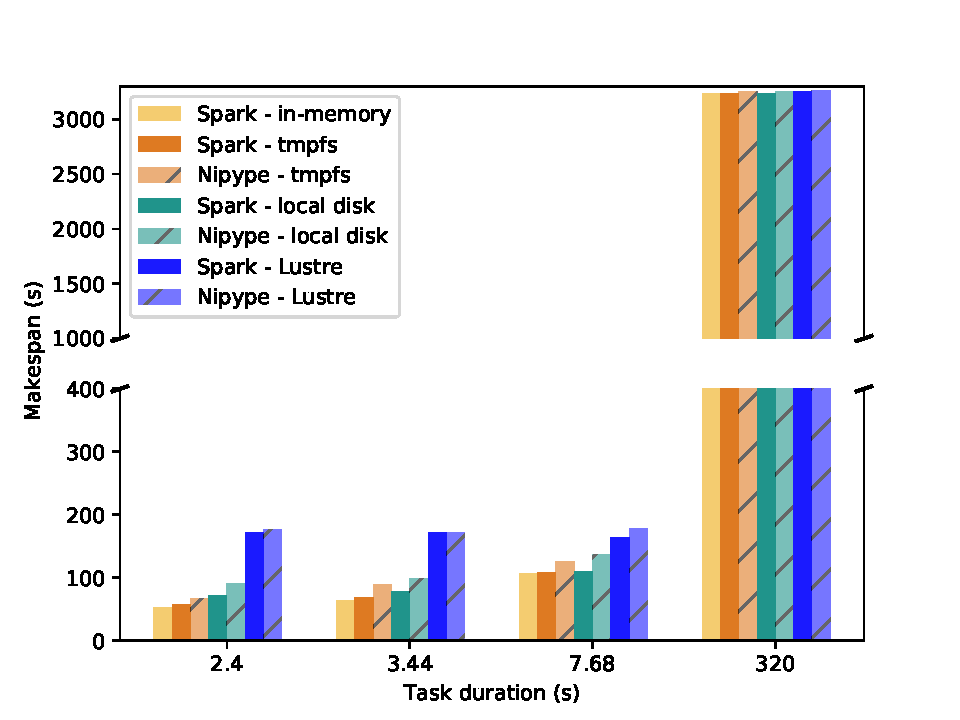
\includegraphics[width=\linewidth]{figures/inmem/cputime.pdf}
    \caption{Experiment 2: complete BigBrain, 125 chunks, 10
    iterations.}\label{fig:inmem:cputime}
\end{subfigure}
\begin{subfigure}{0.5\columnwidth}
    \centering
    \captionsetup{width=.85\linewidth}
    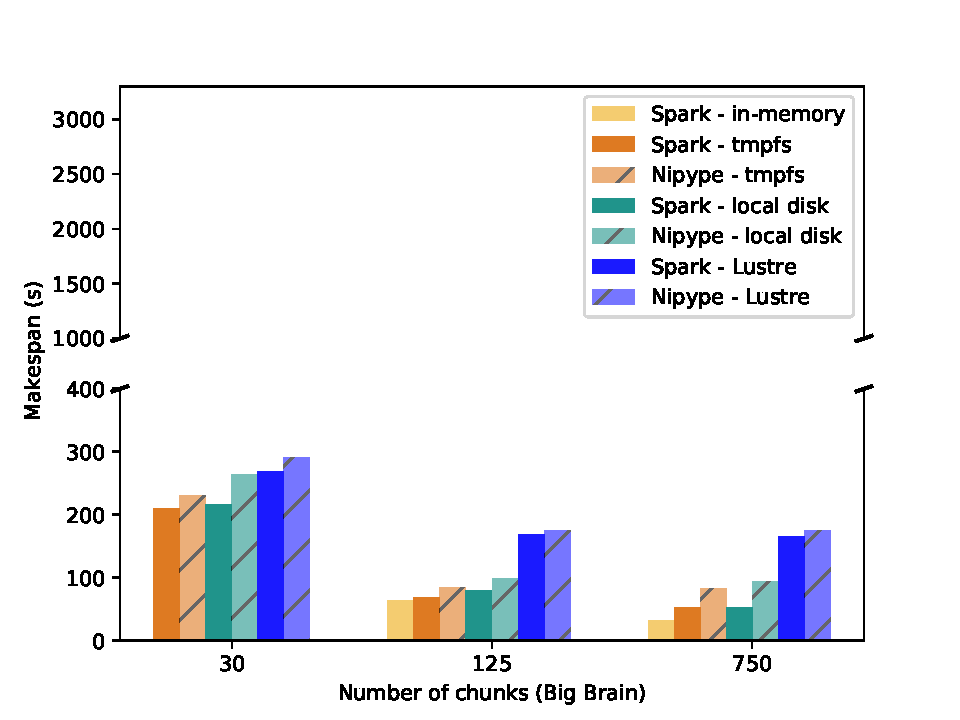
\includegraphics[width=\linewidth]{figures/inmem/numchunks.pdf}
    \caption{Experiment 3: complete BigBrain, 10 iterations, C=
    4,400s.}\label{fig:inmem:numchunks}
\end{subfigure}
\begin{subfigure}{0.5\columnwidth}
    \centering
    \captionsetup{width=.85\linewidth}
    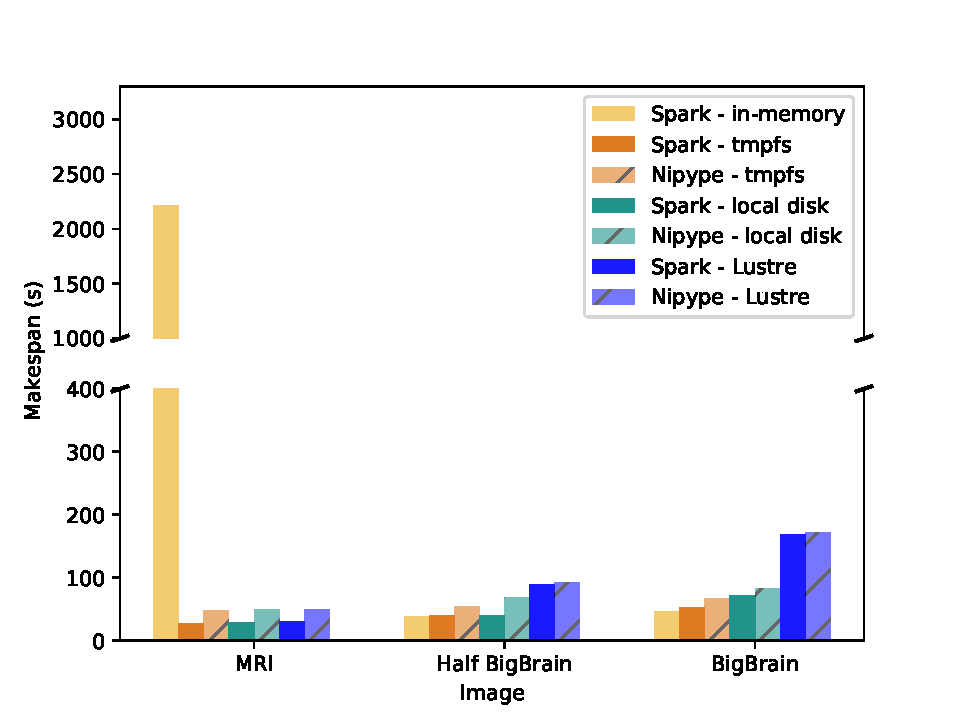
\includegraphics[width=\linewidth]{figures/inmem/datasize.pdf}
    \caption{Experiment 4: 125 chunks, 10 iterations, 1.76-second
    tasks.}\label{fig:inmem:datasize}
\end{subfigure}
\setlength{\belowcaptionskip}{-10pt}
\caption{Experiment results: Makespans of Spark and Nipype writing to memory, tmpfs, local disk and Lustre.}
\label{fig:inmem:results}
\end{figure*}
\subsection{Experiment 1: Number of Iterations}

Fig.~\ref{fig:inmem:iterations} shows the difference between the different file system
choices given varying number of iterations. At 1 iteration, all file systems
behave the same, although the application was writing faster than the disk
bandwidth. This is because application data was not saturating the page cache
(transient phase). The page cache, on Zenith, occupies 40\% of total memory.
With 192~GB of RAM on each node, 76.8~GB of dirty data could be held in a node's
page cache at any given time. As the total amount of data written by the
application increases to 750~GB, there is a greater disparity between Lustre and
in-memory (2.67$\times$ slower, on average). Local disk performance, however, is still
comparable to memory (1.38$\times$ slower, on average). Despite local disk and Lustre
both being in transient state, local disk encounters less contention than what
would be found on Lustre. 

At 100 iterations, or 7,500~GB, Lustre can be found to be, on average, 3.82~x
slower than Spark in-memory. The slowdown experienced can be explained by the
smaller percentage of total data residing in the page cache at a given time,
compared to 10 iterations. Therefore, the effects of Lustre bandwidth are more
significant in this application. At 100 iterations, the application was writing
500GB per node (7,500 GB / 15 nodes) and hence could not run on tmpfs or local
disk.

While there is some variability that can be seen in Fig.~\ref{fig:inmem:iterations}
between the two engines, this believed to be insignificant, and potentially due
to SLURM node allocation delays in our launching of Nipype.

% Comment on the general trend

\subsection{Experiment 2: Task Duration}
% Comment on the general trend We can't really say that imaging tasks are not
% small. Even Freesurfer could be decomposed.
%

Increasing task duration ensured that all file systems had a comparable
performance (Fig.~\ref{fig:inmem:cputime}). Lustre, for instance, is approximately
1.01$\times$ slower than Spark in-memory at a task duration of 320 seconds, whereas it
is approximately 3.25$\times$ slower that Spark in-memory with 2.4 second tasks. This
pattern corroborated our page-cache model which postulates that data movement
costs will have little impact on compute-intensive tasks. The reasoning behind
this is that longer tasks give the page cache more time to flush between disk
writes.

\subsection{Experiment 3: Image Block Size}

% Comment on the general trend
As can be seen in Fig.~\ref{fig:inmem:numchunks}, makespan decreases with increasing
number of chunks. This is due to the fact that parallelism increases with an
increase in number of chunks. At 30 chunks, only 2 CPUs per node are actively
working. At 125 chunks, this changes to a maximum of 9 CPUs per node, and at 750
chunks, up to 40 CPUs can be active.

Due to a size limitation of 2~GB imposed on Spark partitions, Spark with
in-memory computing processing 30 chunks was not performed.

Local disk and tmpfs perform comparably for all conditions, with Lustre being
significantly slower. As with varying the number of iterations, Lustre is slower
due to increased file system contention, which is, at minimum, 15$\times$ greater than
contention on local disk, due to the number of nodes used. With an increase in
number of chunks, local disk and tmpfs makespans begin to converge. A potential
explanation for this may be that tmpfs is utilizing swap space. As concurrency
increases, the memory footprint of the application also increases. It is
possible that at 750 chunks, swapping to disk is required by tmpfs, thus
resulting in similar processing times as local disk.


Swapping may also be an explanation for the variance between Spark in-memory and
tmpfs performance. While Spark may also spill to disk, it only does so when data
does not fit in memory. As none of the RDDs generated throughout the pipeline
were cached and all data concurrently accessed could be maintained in-memory,
spilling to disk was not necessary.

\subsection{Experiment 4: Image Size}

% Comment on the general trend
Increasing overall data size decreases performance, as can be seen in
Fig.~\ref{fig:inmem:datasize}. When the data size is very small (e.g. MRI image) all
file system makespans are comparable. This is due to the fact that page cache
can be leveraged fully regardless of file system. However, this time, Spark
in-memory performed significantly worse than all other file systems, with a
makespan of 2,211 seconds. Upon further inspection, it appeared that Spark
in-memory executed in a sequential order, on a single worker node. Lack of
parallelism for the MRI image may be a result of Spark's maximum partition size,
which is by default 128~MB -- significantly larger than the 13~MB MRI image. 

At half BigBrain, the makespan differences become apparent in both local disk
and Lustre, with Lustre becoming 2.4$\times$ slower than in-memory. This can be
attributed to page cache saturation, as predicted by the model for both half the
BigBrain image and the complete BigBrain. Only the MRI image was predicted to
fall within the model constraints. 

When the complete BigBrain is processed, the disparity between the different
file systems becomes even greater. Lustre becomes 3.68$\times$ slower, whereas local
disk becomes 1.68$\times$ slower. An explanation for this is that the page cache fills
up faster due to data size.

\subsection{Page Cache Model Evaluations}
\begin{figure*}
\begin{subfigure}{0.5\linewidth}
\centering
    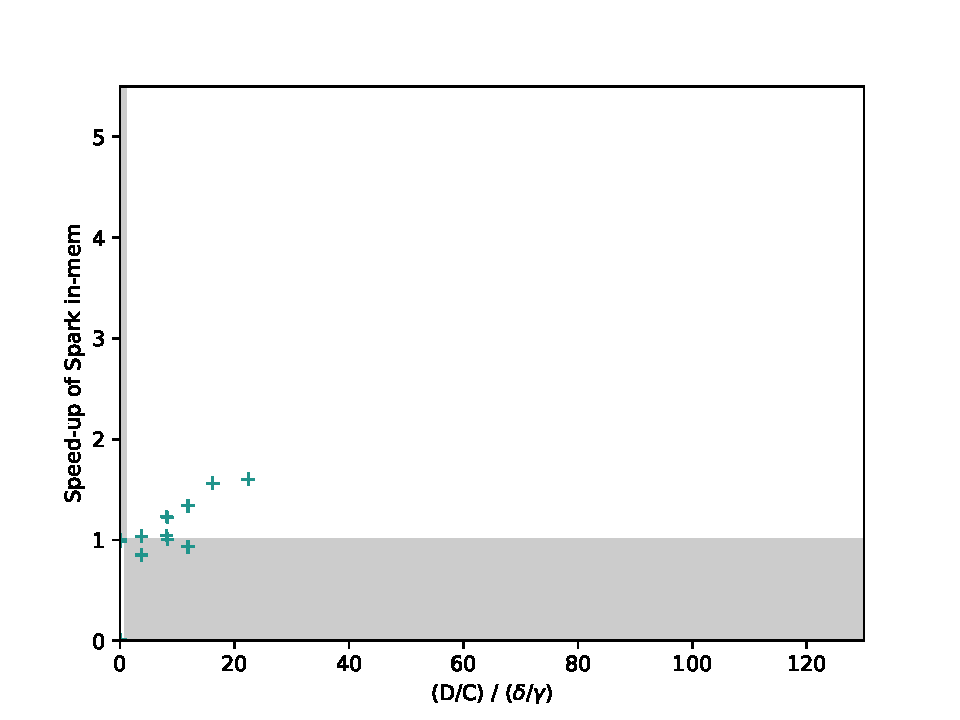
\includegraphics[width=\textwidth]{figures/inmem/local-incrementation.pdf}
\caption{Local Disk}
\label{fig:inmem:modeleval-local}
    \end{subfigure}%
\begin{subfigure}{0.5\linewidth}
\centering
    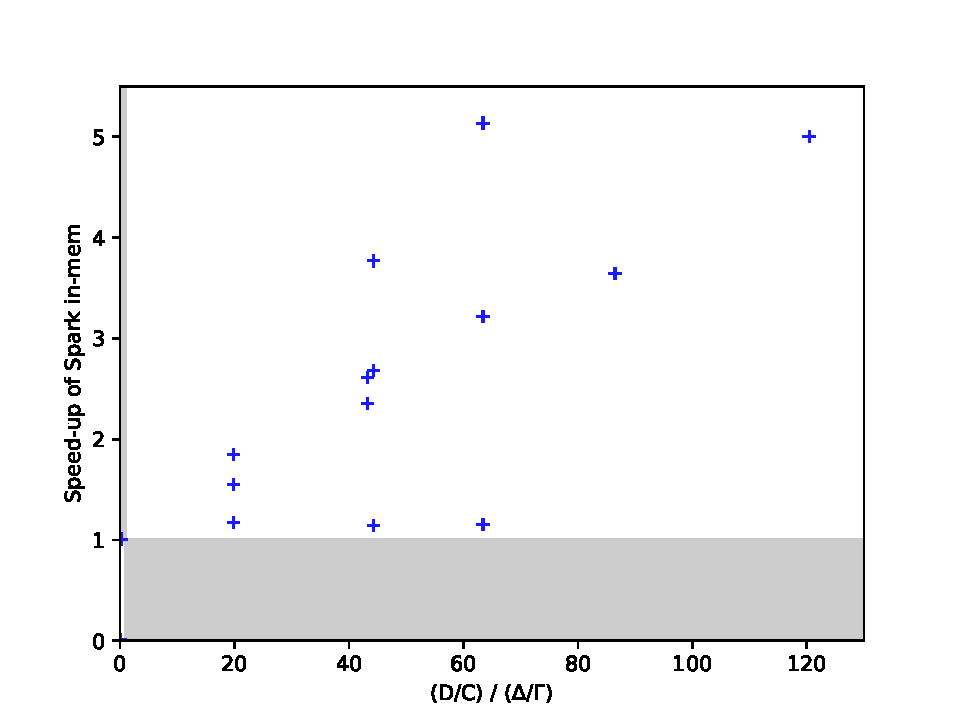
\includegraphics[width=\textwidth]{figures/inmem/lustre-incrementation.pdf}
\caption{Lustre}
\label{fig:inmem:modeleval-lustre}
\end{subfigure}
\setlength{\belowcaptionskip}{-10pt}
    \caption{Page cache model evaluation. Grey regions denote areas that violate
             model predictions.}
\label{fig:inmem:modeleval}
\end{figure*}

In order to evaluate the page cache model, we compared the observed speedup
ratio provided by in-memory computing to the (D/C) / ($\delta$/$\gamma$) and
(D/C) / ($\Delta$/$\Gamma$) ratios (Fig.~\ref{fig:inmem:modeleval}). Speed-up ratios
were computed as the ratio between the makespan obtained with Spark on local
disk or Lustre, and the makespan obtained with Spark for in-memory computing.
Experiments for which there were no in-memory equivalent (i.e. BigBrain split
into 30 chunks) were not considered.

Results show that, overall, the model correctly predicted the effect of page
cache on processing times for local disk and Lustre. That is, the speed-up
provided by in-memory computing was larger than 1 for D/C rates larger than
$\delta/\gamma$ (local disk) or $\Delta/\Gamma$ (Lustre). Conversely, the
speed-up provided by in-memory computing remained close to 1 for D/C rates
smaller than $\delta/\gamma$ (local disk) or $\Delta/\Gamma$ (Lustre). The two
points close to the origin correspond to the sequential processing of the MRI
image by Spark mentioned previously.

Points which violated model predictions were found at 1 iteration, where page
cache would not have been saturated in spite of a high D/C (transient state).
However, in all cases, the ``1" boundary was never trespassed by more than a
factor of 0.19, and is therefore likely a result of system variability.

\section{Discussion} % 2 pages
\label{sec:inmem:discussion}

\subsection{Effect of In-Memory Computing}
% Shared fs vs local disk vs in-memory: what do we gain?
We measured the effect of in-memory computing by comparing the runs of Spark
in-memory (yellow bars in Fig.~\ref{fig:inmem:results}) to the ones of Spark on local
disk (non-hatched green bars). The speed-up provided by in-memory computing is
also reported in Fig.~\ref{fig:inmem:modeleval-local}. The speed-up provided by
in-memory computing increases with (D/C) / ($\delta$/$\gamma$), as expected from
the model. In our experiments, it peaked at 1.6, for a ratio of 16.2. This
corresponds to the processing of the BigBrain with 125 chunks and 1.76-second
tasks in experiment 4 (total computing time C=2,200s), which is typically
encountered in common image processing tasks such as denoising, intensity
normalization, etc. The speedup of 1.6 is also reached with a ratio of 22.7 in
experiment 3, obtained by processing the BigBrain with 750 chunks.

The results also allow us to speculate on the effect of in-memory computing on
the pre-processing of functional MRI, another typical use case in neuroimaging.
Assuming an average processing time of 20 minutes per subject, which is a
ballpark value commonly observed with the popular
\href{https://www.fil.ion.ucl.ac.uk/spm/}{SPM} or
\href{https://fsl.fmrib.ox.ac.uk/fsl/fslwiki/}{FSL} packages, an input data size
of \SI{100}{\mega\byte} per subject, and an output data size of \SI{2}{\giga\byte} (20-fold increase compared
to input size), the D/C rate would be 1.8MB/s, which would reach the
$\delta/\gamma$ threshold measured on this cluster for $\gamma=108$, that is, if
108 subjects were processed on the same node. This is very unlikely as the
number of CPUs per node was 40. We therefore conclude that in-memory computing
is likely to be useless for fMRI analysis. Naturally, this estimate is strongly
dependent on the characteristics of the cluster.

\subsection{Effect of Data Locality}

We measure the effect of data locality by comparing the runs of Spark on local
disk (non-hatched green bars in Fig.~\ref{fig:inmem:results}) to the ones of Spark on
Lustre (non-hatched blue bars). The speed-up provided by local execution peaked
at 3.2, for 750 chunks in experiment 3. Overall, writing locally was usually
preferable over writing to Lustre, as a result of the lower contention on local
disk. Although it may be true that network bandwidths exceed that of
disks~\cite{ananthanarayanan2011disk}, locality remains important as contention
on a shared file system tends to be much higher than on local disk. The only time
writing locally did not have significant impact over Lustre was in experiments 1
and 4, at 1 iteration and when processing the MRI image, respectively. In both
these scenarios, the Lustre writes did not impact performance as the data was
able to be written to page cache and flushed to Lustre asynchronously.

\subsection{Combined Effect of In-Memory and Data Locality}
We measure the combined effect of data locality and in-memory computing by
comparing the runs of Spark in-memory (yellow bars in Fig.~\ref{fig:inmem:results}) to
the ones of Spark on Lustre (non-hatched blue bars). The speed-up provided by
the combined use of data locality and in-memory computing is also reported in
Fig.~\ref{fig:inmem:modeleval-lustre}. The provided speed-up increases with (D/C) /
($\Delta$/$\Gamma$), as expected from the model. In our experiments, it peaked
around 5, for ratios of 120.4 and 64. Again, this configuration is likely to
happen in typical image processing tasks performed on the BigBrain.

As for the fMRI speculation, the D/C rate of 1.8MB/s would reach the
$\Delta/\Gamma$ threshold for $\Gamma=280$, which is a realistic number of
subjects to process on a complete cluster. Naturally, this estimate is highly
dependent on the observed bandwidth of the shared file system ($\Delta$).

\subsection{Effect of Lazy Evaluation}

The effects of lazy evaluation can be seen throughout the experiments. Nipype
was found to be slower than Spark in most experiments. While the Nipype
execution graph is generated prior to workflow execution, there are no
optimizations to ensure that the least amount of work is performed to produce
the required results. 

During the processing of Experiment 3, 750 chunks were processed in two batches
for both Spark and Nipype due to CPU limitations. Rather than running each
iteration on the full dataset, as with Nipype, Spark opted to perform all the
iterations on the first batch (load, increment, save), and then proceeded to
process the second batch. Such an optimization is important, even when
processing data on disk, as it would presumably increase the occurrence of cache
hits. This may partially explain the speedup seen at 750 chunks in
Figure~\ref{fig:inmem:numchunks}.% Spark local vs nipype local: presumably increases cache hits

\subsection{Can tmpfs and Page Caches Emulate In-Memory Computing?}
% tmpfs and local disks fill up: need cleanup. Can we emulate in-memory
% computing using write buffers or tmpfs?

Although tmpfs and page cache do improve performance, as seen in
Figure~\ref{fig:inmem:results}, they do not always perform equivalently to in-memory.
Tmpfs's main limitation is that data residing on it may be swapped to disk if
the system's memory usage is high. When it reaches this point, its performance
slows down to swap disk bandwidth, as observed in Figure~\ref{fig:inmem:datasize}.
Page cache suffers a similar dilemma. I/O blocking writes to disk occur when a
given percentage (e.g. 40~\%) of total memory is occupied by dirty data. When
the threshold is exceeded, processes performing writes must wait for dirty data
to be flushed to disk.

Furthermore, like memory, tmpfs and page cache are shared resources on a node.
If users on the node are heavily using memory to incite tmpfs to writes to swap
space, or are performing data-intensive operations that fill up the page cache,
tmpfs/page cache performance on will be limited for other users. However, it is
possible to request through the HPC scheduler a certain amount of available
memory. Ultimately, in-memory data will also need to be spilled to disk if
memory usage exceeds amount of available memory, although disk writes are likely
to occur in tmpfs and page cache before requested available memory is filled.

\subsection{Scheduling Remarks}

A common recommendation in Spark is to limit the number of cores per executors
to 5, to preserve a good I/O throughput (see
\href{http://blog.cloudera.com/blog/2015/03/how-to-tune-your-apache-spark-jobs-part-2}{Cloudera
blog}), but the rationale for this recommendation is hardly explained. We
believe that throughput degradation observed with more than 5 cores per executor
might be coming from full page caches.

Spark does not currently include any active management of disk I/Os or page
caches. We believe that it would be beneficial to extend it toward this
direction, to increase the performance of operations where local storage has to
be used, such as disk spills or shuffles. For instance, workflow-aware cache
eviction policies that maximizes page cache usage for the workflows could be
investigated. 

An alternative Nipype plugin designed for running on Slurm was not used in the
experiments. The Slurm plugin requests a Slurm allocation for each processed
data chunk. Such a scheduling strategy was not ideal in our environment where
oversubscription of nodes was not enabled.

Unlike Spark, Nipype by default opts to use all available CPUs rather than to
load balance data across the cluster. That is, given 50 chunks and 40 cores,
Spark will only use up 25 cores and process in two batches. Nipype will also
have no choice but to split up the processing into two batches, but will first
process 40 chunks, immediately followed by the remaining 10. While both are
reasonable strategies for data processing, Spark may end up benefiting more from
the page cache, as less data is written in parallel (25 vs 40), giving more time
for the page cache to flush.

Nipype's MapNodes, which apply a given function to each element in a list, were
found to be slower than the Node, which apply a function to a single element,
due to a blocking mechanism. For this reason, we selected to iterate through a
series of Nodes in our code despite MapNodes being easier to use.

% \todo{If time permits, it would be useful to say that we checked that
% scheduling between both engines was similar, and show two Gantt charts to
% justify that.}

\subsection{Other Comments}

Writing to node-local storage in a cluster environment comes at a cost, for both
Nipype and Spark without HDFS. When a node is lost, the node-local data is lost
with it. While Spark will recompute the lost partition automatically using
lineage, Nipype will fail for all tasks requiring the data. Nevertheless, Spark
will also fail if RDDs of node-local filenames are shuffled, as the data
associated to the filenames will not be shuffled with the RDD and there will be
no mechanism in place to fetch it.

When executed on Lustre, Nipype will checkpoint itself, ensuring resumption from
last checkpoint during re-execution. This is particularly important in the case
of compute-intensive applications, such as those found in neuroimaging. Spark
also provides a checkpointing mechanism, however, it requires HDFS.

It is common in neuroimaging applications for users to want access to all
intermediate data. Such a feature is currently only possible when writing to
shared file system. It would also not be an option with Spark in-memory. To
enable this, burst buffers or heterogeneous storage managers (e.g.
Triple-H~\cite{islam2015triple}) could be used to ensure fast processing and
that all outputs (including intermediate outputs) will be sent asynchronously to
the shared file system.

It was expected that Spark would experience longer processing times,
particularly with the small datasets, due to Java serialization. This was not
found to be the case. Unlike Spark, Nipype performs a more thorough provenance
capture, potentially owing to longer processing times.

In this paper, we analysed the effects of Big Data strategies on an map-only
artificial neuroimaging pipeline. This allowed us to examine the effects of
these strategies without being significantly obscured by other conditions.
Studying the effects of such strategies on map-reduce type workflows, in
addition to real neuroimaging pipelines, would allow us to gain further insight
on the added value of the Big Data performance strategies for neuroimaging use
cases remains to be done.

\section{Conclusion} % 1 page with refs
\label{sec:inmem:conclusion}

Big Data performance optimization strategies help improve performance of typical
neuroimaging applications. Our experiments indicate that overall, in-memory
computing enables greater speedups than what can be obtained by using page cache
and tmpfs. While page cache and tmpfs do give memory-like performance, they are
likely to fill up faster than memory, leading to increased performance penalties
when compared to in-memory computing. We conclude that extending Big Data
processing engines to better support neuroimaging applications, including
developing their provenance, fault-tolerance, and reproducibility features, is
worthwhile.

Data locality plays an important role in application performance. Local disk was
found to perform better than the shared file system despite having lower
bandwidth, due to increased contention on the shared file system. Since local
disk typically has less contention than shared file systems, it is recommended to
store data locally. However, using local storage without a distributed file
system may limit fault tolerance.

Although a more thorough analysis of lazy evaluation remains to be performed, it
is speculated that this may be the cause of the general performance difference
between Spark and Nipype. Furthermore, it was found that lazy evaluation
optimizations increase the likelihood of cache hits, thus improving overall
performance.

Even though Big Data strategies are beneficial to the processing of large
images, it is estimated that it would require running a functional MRI dataset
with 280 concurrent subjects for any noticeable impact using our Lustre
bandwidth estimate. Benchmarking Spark and Nipype using such a large fMRI
dataset would be a relevant follow-up experiment, to test this hypothesis. It
would also be useful to evaluate other types of applications, such as ones
containing data shuffling steps.

Finally, we plan to extend this study by including task scheduling strategies in
a multi-tenant environment. We expect to observe important differences between
Spark and Nipype, due to Spark's use of overlay scheduling. The impact of other
Big Data technologies, such as distributed in-memory file
systems(e.g.~\href{https://ignite.apache.org}{Apache Ignite}) and Lustre
scalability issues~\cite{sparkhpc}, could also be investigated.